\begin{problem}
Implement the Bernstein approximation operator for arbitrary degree $n$ and use it to find an approximation to $f(x) = \lvert x - 1/2 \rvert$ in $[0,\, 1]$ with an accuracy of $10^{-3}$. Plot the function and its approximation.
\end{problem}

\begin{solution}
As we know, the convergence of the Bernstein polynomial approximation is very slow, therefore we need really high degree polynomials in order to achieve the desired accuracy. We first tried programing the algorithm as it is with the binomial coefficient in its expanded form, that is:
\begin{equation*}
\frac{n!}{k!(n-k)!}
\end{equation*}
However with this approach we only reached an accuracy of 0.0258 as we can not compute directly factorials of large numbers (crashed at $n = 172$). Then we turned to compute the binomial coefficients with MATLAB's built in \texttt{nchoosek} function, this did a better job, lowering the error to 0.008, but this is still not enough. We also tried to use some properties of the binomial coefficient, namely:
\begin{align*}
\binom{n}{k} &= \frac{n}{k}\binom{n-1}{k-1} \\
\binom{n}{k} &= \binom{n}{n-k} \\
\binom{n}{0} & = 1
\end{align*}
but we did not get a significant improvement over MATLAB's implementation.
\begin{figure}[h]
\centering 
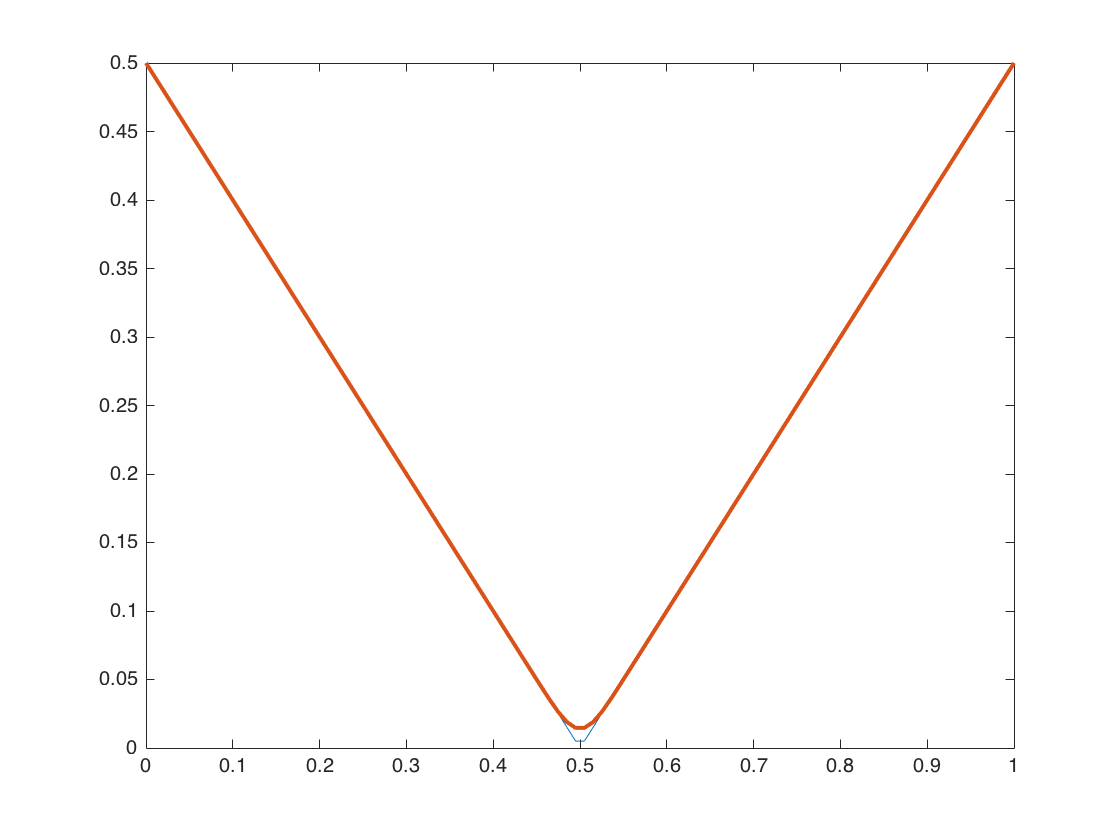
\includegraphics[scale = 0.25]{task2hw3.png}
\caption{Bernstein approximation to $f(x) = \lvert x-1/2 \rvert$ with an accuracy of $10^{-2}$}
\label{task2hw3fig}
\end{figure}
\end{solution}